\documentclass[simplex.tex]{subfiles}
% NO NEED TO INPUT PREAMBLES HERE
% packages are inherited; you can compile this on its own

\onlyinsubfile{
\title{NeuroData SIMPLEX Report: Subfile}
}

\begin{document}
\onlyinsubfile{
\maketitle
\thispagestyle{empty}

The following report documents the progress made by the labs of Randal~Burns and Joshua~T.~Vogelstein at Johns Hopkins University towards goals set by the DARPA SIMPLEX grant.

%%%% Table of Contents
\tableofcontents

%%%% Publications
\bibliographystyle{IEEEtran}
\begin{spacing}{0.5}
\section*{Publications, Presentations, and Talks}
%\vspace{-20pt}
\nocite{*}
{\footnotesize	\bibliography{simplex}}
\end{spacing}
%%%% End Publications
}

\subsection{Robust Law of Large Graphs}

To estimate the mean of a collection of weighted graphs under a
low rank random graph model (e.g. Stochastic Blockmodel) when
observing contaminated graphs, we propose an estimator which not
only inherits robustness from element-wise robust estimators but
also has small variance due to application of a rank-reduction
procedure. Under appropriate conditions, we prove that our
estimator outperforms standard estimators via asymptotic relative
efficiency.  And we illustrate our theory and methods by Monte
Carlo simulation in figure~\ref{fig:rlolg}.

\begin{figure}[h!] 
\begin{cframed} 
\centering
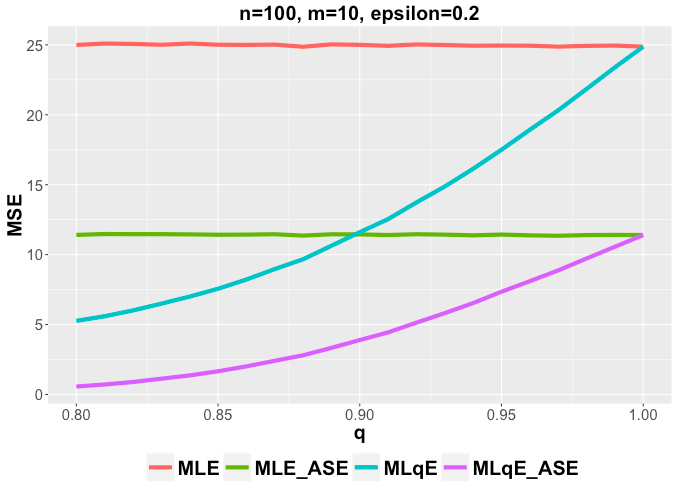
\includegraphics[width=0.45\textwidth]{./figs/robQ.png}
\hspace{6pt}
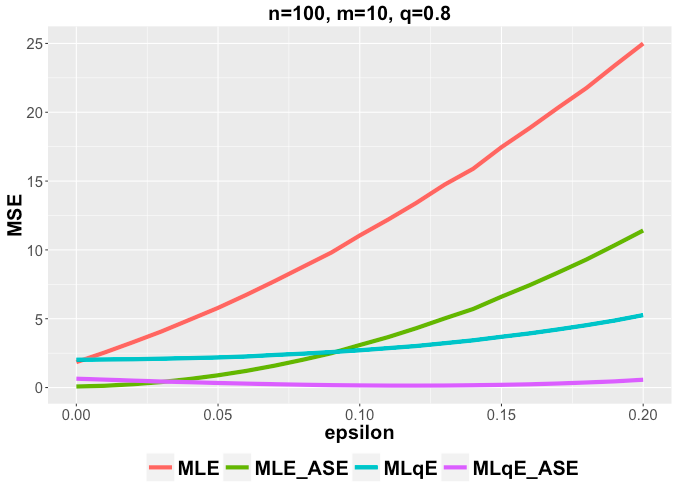
\includegraphics[width=0.45\textwidth]{./figs/robEps.png} 
\caption{
For the figure on the left, we vary the proportion of the contamination
represented by  and conclude: \textbf{1. MLE (red) vs ML$q$E 
(blue)}: MLE outperforms a little bit when there is no
contamination, but it degrades dramatically when contamination
increases; \textbf{2. MLE (red) vs MLE\_ASE (green)}: MLE\_ASE wins
the bias-variance tradeoff; 
\textbf{3. ML$q$E  (blue) vs MLE\_ASE (purple)}: 
MLE\_ASE wins the bias-variance tradeoff; 
\textbf{4.  ML$q$E\_ASE (purple) vs MLE\_ASE (green)}: 
When contamination is large enough, ML$a$E\_ASE is better, since it 
inherits the robustness from ML$q$E.  For the right panel, we vary 
the parameter $q$ in the ML$q$E.  Note that when $q=1$, ML$q$E becomes 
MLE so that the curves intersect. As $q$ decreases, we intend to have 
more bias but still win the bias-variance trade-off by reducing the variance.
}
\label{fig:rlolg} 
\end{cframed}
\end{figure}



Also, to get the convergence rate of the variance of ML$q$E, we
proved: 1. the uniform convergence $\sup_{\theta \in \Theta} \left|
E_f[g(X, \theta)] − \frac{1}{m} \sum_{i=1}^m g(X_i, \theta) \right| \to
0$ as $m \to \infty$, where $g(x, \theta)$ is the equation for
ML$q$E; 2. There exists at least one population solution of the
ML$q$E equation which is smaller than the expectation of the MLE.

In summary, MLE outperforms a little bit when there is no contamination,
but it degrades dramatically when contamination increases while ML$q$E
still does a good job. Applying ASE to either entry-wise MLE or
entry-wise ML$q$E reduces the variance by bias towards the low rank
approximation. Our estimator based on ASE of ML$q$E inherits the
robustness from ML$q$E, and it has low variance. When contamination is
large enough, our estimator performs the best among all the four.


We tested our algorithm’s performance on a synthetic dataset based on
structural connectomic data. The graphs are based on diffusion tensor MR
images collected and available at the Consortium for Reliability and
Reproducibility (CoRR). It contains 454 different brain scans, each of
which was processed to yield an undirected, weighted graph with no
self-loops, using the ndmg pipeline..  The vertices of the graphs
represent different regions in the brain defined according to an atlas.
We used the  CPAC200 atlas with 200 vertices. The weight of an edge
between two vertices represents the number of white-matter tract
connecting the corresponding two regions of the brain. In order to
evaluate the performance of the two estimators, we used a cross
validation on the 454 graphs of each size. Specifically, for a given
atlas, each Monte Carlo replicate corresponds to sampling m graphs out
of the 454 and computing the four estimates using the m selected graphs.
We then compared these estimates to the sample mean for the remaining
454-m adjacency matrices.  We ran 1000 simulations on the CPAC200
atlases for both sample size $M=2, 5$.  We also considered all possible
dimensions for adjacency spectral embedding by ranging d from 1 to n in
order to investigate the impact of the dimension selection procedures.
We plot the result in the following figure.


\begin{figure}[h!]
\begin{cframed}
\centering
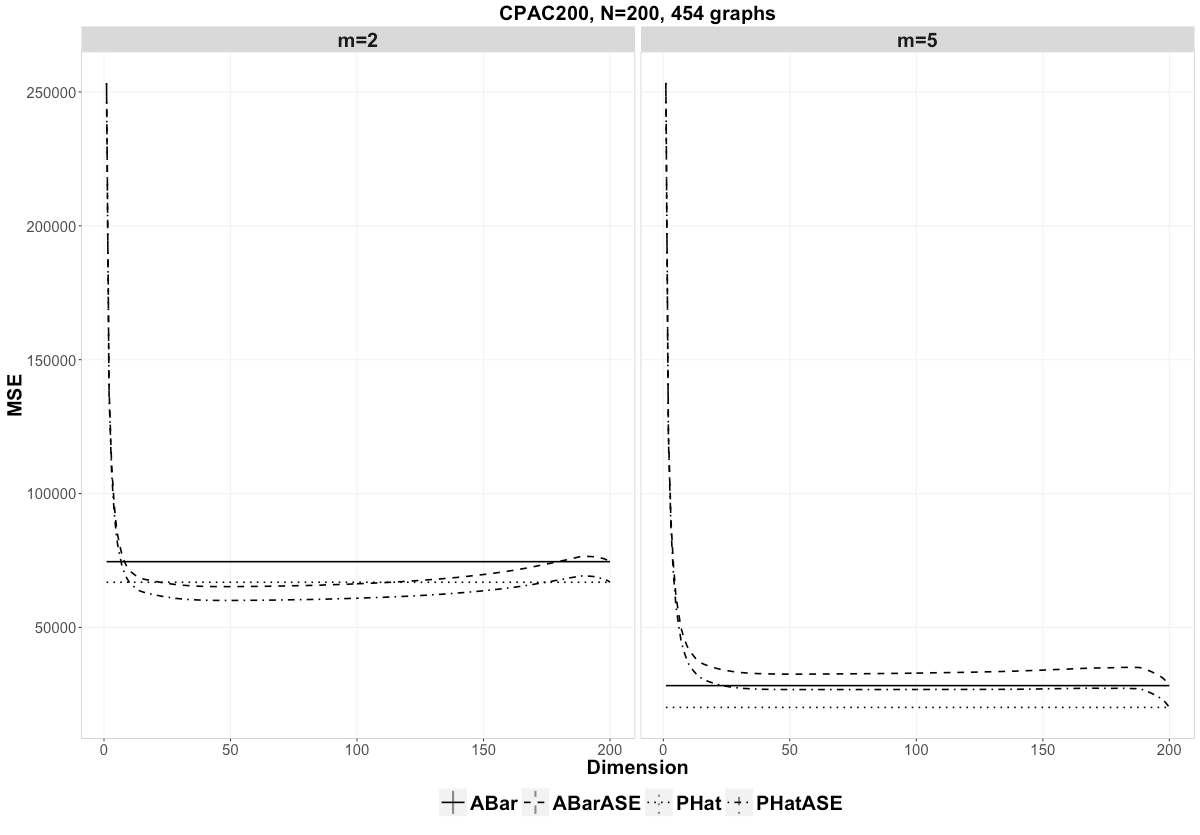
\includegraphics[width=\textwidth]{./figs/robDim.png}
\caption{
{\bf Comparison of MSEhat of the four estimators for the CPAC200 atlases at two sample sizes for the CoRR data.}  
For the figure on the left, we examine the four estimators at sample size m=2. 
{\bf 1. MLE (horizontal solid line) vs MLqE (horizontal dotted
line):} 
ML$q$E outperforms MLE since
robust estimators are always preferred in practice;
{\bf 2. MLE (horizontal solid line) vs MLE\_ASE (dashed line):} MLE\_ASE wins the bias-variance
tradeoff when embedded into a proper dimension; 
{\bf 3. MLqE (horizontal
dotted line) vs ML$q$E\_ASE (dashed dotted line):}
ML$q$E\_ASE wins the
bias-variance tradeoff when embedded into a proper dimension; 
{\bf 4.  ML$q$E\_ASE (dashed dotted line) vs MLE\_ASE (dashed
line):}
MLqE\_ASE is better, since it inherits the robustness from 
ML$q$E. For the figure on the right, we still can see the
robustness but the lack of low-rankness
for a larger number of samples degrades the effect of ASE.
}
\label{fig:robDim}
\end{cframed}
\end{figure}


\end{document}
